% Provenance (never printed): see sources/outline_sources.md (Year 1: hotspots and
% mantle plumes; hotspot chains and absolute plate motion; large igneous provinces).
% Hotspot map, pole fit, rates and swell from figdata/bachelor-1/hotspots.py (data
% data/derived/bachelor-1-hotspots.csv, Table 1 of the Morgan and Morgan 2007 electronic
% supplement); exercise and problem values in the Book 3 scratch calculators calc/ch15.py and
% calc/ch15ex.py. "Hotspot" is re-founded from Book 1 (g7 volcanoes), "hotspot track"
% from Book 2 (g11 plate-motions); Book 2 owns the age--distance fit of the Hawaiian
% chain, so this chapter fits the Pacific Euler pole from track directions instead.
\chapter{البقع الساخنة والبراكين داخل الصفائح}\label{ch:b1:hotspots}

منذ يناير 1983، وعلى مدى عقود بعدها، ثارت كيلاويا، في جزيرة هاواي، دون انقطاع تقريبًا من فوهة على منطقة شقّها الشرقي، فأفرغت نحو \qty{0.12}{km^3} من الحمم كل سنة. وتقف كيلاويا في وسط صفيحة المحيط الهادئ، على آلاف الكيلومترات من أيّ حيد أو خندق. وإلى الشمال الغربي تصبح جزر هاواي أقدم فأقدم، ثم تغوص تحت البحر، وتمتد السلسلة كخطّ من براكين غارقة لآلاف الكيلومترات أخرى. تفسّر تكتونية الصفائح البراكين عند حدود الصفائح؛ وهذا الفصل يتناول ما لا تفسّره مباشرةً، أي \omterm{def:b1:hotspots:hotspot}{البقع الساخنة}، وما تقوله في المقابل: كيف تتحرك الصفائح فوق \omterm{def:b1:layered-earth:layers}{الوشاح} العميق، وكم من الحرارة والصخر يصعد من الأسفل، وكيف صُنعت بعض الفيضانات الهائلة للحمم، أي المقاطعات البركانية الكبرى.
% ledger: pp1801:kilauea-rate

\begin{recall}
\omterm{def:b1:hotspots:hotspot}{البقعة الساخنة} تغذّي البراكين من أعماق \omterm{def:b1:layered-earth:layers}{الوشاح} بينما تتحرك الصفيحة فوقها، والصفيحة تحمل معها \omterm{def:b1:hotspots:track}{أثر البقعة الساخنة} الذي تكون براكينه أقدم كلما بَعُدت (الكتاب 1، الصف 7؛ الكتاب 2، الصف 11). وصفيحة تدور \omterm{def:b1:plate-kinematics:euler-pole}{بمتجهة أويلر} $\vec\omega$ تتحرك بسرعة $\vec v = \vec\omega\times\vec r$، أي بسرعة $\omega R\sin\Delta$، عمودية على \omterm{def:b1:spherical-astronomy:spherical-triangle}{الدائرة العظمى} التي تصلها بالقطب (\cref{ch:b1:plate-kinematics})؛ والتضاريس مرفوعة \omterm{def:b1:isostasy-gravity:isostasy}{بالتوازن الأيزوستاتي} (\cref{ch:b1:isostasy-gravity})؛ والصخر الدافئ أخفّ بالكسر $\alpha\,\Delta T$ (\cref{ch:b1:rifts-ridges-margins}).
\end{recall}

\section{البقع الساخنة وأعمدة الوشاح}\label{sec:b1:hotspots:plumes}

\begin{definition}[البقعة الساخنة]\label{def:b1:hotspots:hotspot}
\emph{البقعة الساخنة}\index{البقعة الساخنة} منطقة بركانية لا يتعلّق موضعها بحدود الصفائح، نشطة على مدى عشرات الملايين من السنين، ويُعتقد أنها تتغذّى من \omterm{def:b1:layered-earth:layers}{وشاح} أحرّ من \omterm{def:b1:layered-earth:layers}{الوشاح} المحيط بها.
\end{definition}

يتوقف عدد \omterm{def:b1:hotspots:hotspot}{البقع الساخنة} على ما يُحسب. فجدول \omterm{def:b1:hotspots:hotspot}{البقع الساخنة} المستعمل في هذا الفصل يذكر 68 منها، لكن مؤلفيه يهملون عدة معالم يرون أنها لا تسجّل حركة صفيحة، ويصنّفون بعضًا مما يبقونه على أنه محتمل فقط. وبعض \omterm{def:b1:hotspots:hotspot}{البقع الساخنة}، ومنها هاواي وأيسلندا وريونيون، لها أثر طويل منتظم وإنتاج كبير، كما ينتظر من مصدر عميق؛ وأخرى صغيرة وقصيرة العمر. وتقذف معظم براكين \omterm{def:b1:hotspots:hotspot}{البقع الساخنة} البازلت؛ وحيث تقع البقعة تحت قارة، يذيب البازلت الحار \omterm{def:b1:layered-earth:layers}{القشرة}، وتتحول الثورانات العظيمة إلى ريوليت، كما في يلوستون.
% ledger: mm07:table, data:b3-hotspots, yvo:calderas

\begin{definition}[عمود الوشاح]\label{def:b1:hotspots:plume}
\emph{عمود الوشاح}\index{عمود الوشاح} عمود من صخر وشاحي حار وطافٍ يصعد من طبقة حدّية حرارية عميقة في \omterm{def:b1:layered-earth:layers}{الوشاح}. وللعمود الجديد \emph{رأس} منتفخ كبير على \emph{ذيل} طويل ضيّق، أو قناة؛ وبمجرد أن ينتشر الرأس تحت \omterm{def:b1:layered-earth:lithosphere}{الغلاف الصخري}، يواصل الذيل إيصال المصهور إلى السطح لعشرات الملايين من السنين.
\end{definition}

يأتي الشكل من المختبر. ففي تجارب الخزانات في السبعينيات، صعدت طبقة من مائع خفيف أقل لزوجة من المائع الذي فوقها كجيب مستدير تغذّيه أنبوبة خلفه: فطرة. وينتشر رأس \omterm{def:b1:hotspots:plume}{عمود الوشاح} ويتسطّح عند بلوغه قاعدة \omterm{def:b1:layered-earth:lithosphere}{الغلاف الصخري}؛ فينخفض الضغط، ويذوب الصخر الحار بكميات كبيرة. وتتفق الفيضانات البازلتية مع الصورة: فبراكينها تستمر نحو عشرة ملايين سنة، لكن معظم حجمها يُقذف في نحو مليون سنة أو أقل، وكثيرًا ما تقترن بانفصال قارة (\cref{sec:b1:hotspots:lips}).
% ledger: hist:plumes (Whitehead and Luther 1975), cr03:summary

\begin{omfigure}
\begin{tikzpicture}[font=\scriptsize,
  lbl/.style={fill=white, fill opacity=0.8, text opacity=1, inner sep=1pt, align=center}]
% ---- panel (a): the head arrives ----
\begin{scope}
\clip (0,-5) rectangle (6.4,1.3);
\fill[orange!12] (0,-5) rectangle (6.4,0);
\fill[omSea!45] (0,0) rectangle (6.4,0.55);
\fill[omLithBasalt!55] (0,0) rectangle (6.4,-0.9);
% flood basalt: a stack of flat flows on the sea floor
\fill[black!55] (2.5,0) -- (2.7,0.32) -- (6.1,0.32) -- (6.3,0) -- cycle;
\foreach \y in {0.08,0.16,0.24} \draw[white!70!black, line width=0.3pt] (2.62,\y) -- (6.18,\y);
% plume: tail and flattened head
\fill[red!40] (4.25,-5) -- (4.25,-1.7) -- (4.55,-1.7) -- (4.55,-5) -- cycle;
\fill[red!40] (4.4,-1.45) ellipse[x radius=1.9, y radius=0.55];
\draw[red!60!black, line width=0.4pt] (4.25,-5) -- (4.25,-1.95) (4.55,-5) -- (4.55,-1.95);
\draw[red!60!black, line width=0.4pt] (4.4,-1.45) ellipse[x radius=1.9, y radius=0.55];
% melt rising through the plate
\foreach \x in {3.2,3.9,4.6,5.3}
  \draw[red!75!black, line width=0.6pt, decorate, decoration={snake, amplitude=0.6pt, segment length=3pt}] (\x,-1.1) -- (\x,0.05);
\end{scope}
\draw[black!70] (0,-5) rectangle (6.4,1.3);
\node[lbl, anchor=north west] at (0.1,1.25) {(أ) وصول الرأس};
\node[lbl, anchor=west] at (0.1,-0.45) {الغلاف الصخري};
\node[lbl, anchor=west] at (0.1,0.3) {البحر};
\node[lbl, anchor=south] at (4.4,0.62) {بازلت فيضي (LIP)};
\node[lbl, anchor=east] (ph) at (1.9,-1.75) {رأس العمود};
\draw[black!70] (ph.east) -- (2.7,-1.6);
\node[lbl, anchor=east] at (4.1,-3.6) {ذيل العمود};
\node[lbl, anchor=west] at (0.1,-4.6) {الوشاح};
% ---- panel (b): the plate has moved on ----
\begin{scope}[xshift=6.8cm]
\begin{scope}
\clip (0,-5) rectangle (6.4,1.3);
\fill[orange!12] (0,-5) rectangle (6.4,0);
\fill[omSea!45] (0,0) rectangle (6.4,0.55);
\fill[omLithBasalt!55] (0,0) rectangle (6.4,-0.9);
% the flood basalt, carried away to the left
\fill[black!55] (-0.9,0) -- (-0.7,0.32) -- (1.0,0.32) -- (1.2,0) -- cycle;
\foreach \y in {0.08,0.16,0.24} \draw[white!70!black, line width=0.3pt] (-0.8,\y) -- (1.08,\y);
% the chain: older volcanoes to the left, lower (they sank as the plate cooled)
\fill[black!35] (1.45,0) -- (1.75,0.2) -- (2.05,0) -- cycle;
\fill[black!38] (2.15,0) -- (2.5,0.3) -- (2.85,0) -- cycle;
\fill[black!42] (2.95,0) -- (3.35,0.42) -- (3.75,0) -- cycle;
\fill[black!65] (3.95,0) -- (4.45,0.95) -- (4.55,0.97) -- (5.05,0) -- cycle;
\fill[red!70!black] (4.43,0.93) -- (4.57,0.95) -- (4.5,1.12) -- cycle;
% the plume tail, still in place, and a small spread of hot rock under the plate
\fill[red!40] (4.35,-5) -- (4.35,-1.1) -- (4.65,-1.1) -- (4.65,-5) -- cycle;
\fill[red!40] (4.5,-1.05) ellipse[x radius=0.75, y radius=0.2];
\draw[red!60!black, line width=0.4pt] (4.35,-5) -- (4.35,-1.2) (4.65,-5) -- (4.65,-1.2);
\draw[red!75!black, line width=0.6pt, decorate, decoration={snake, amplitude=0.6pt, segment length=3pt}] (4.5,-0.95) -- (4.5,0.8);
\end{scope}
\draw[black!70] (0,-5) rectangle (6.4,1.3);
\node[lbl, anchor=north west] at (0.1,1.25) {(ب) بعد زمن طويل};
\draw[->, line width=1pt] (3.2,-0.45) -- (1.2,-0.45) node[midway, above=1pt, lbl] {حركة الصفيحة};
\node[lbl, anchor=south] at (0.55,0.38) {المقاطعة (LIP)};
\node[lbl, anchor=south] at (2.7,0.62) {أقدم، منقرض};
\node[lbl, anchor=west] at (5.0,0.95) {بركان\\نشط};
\node[lbl, anchor=east] at (4.2,-3.6) {ذيل العمود};
\node[lbl, anchor=west] at (4.75,-2.6) {يبقى في\\الوشاح};
\end{scope}
\end{tikzpicture}
\par\smallskip{\small نموذج \omterm{def:b1:hotspots:plume}{عمود الوشاح} \omterm{def:b1:hotspots:hotspot}{لبقعة ساخنة} (تخطيطي، غير مرسوم بالمقياس). (أ)~عمود جديد: يتسطّح رأسه تحت \omterm{def:b1:layered-earth:lithosphere}{الغلاف الصخري} ويذوب مع انخفاض الضغط عنه، وتُقذف فيضانات بازلتية، أي مقاطعة بركانية كبرى، خلال بضعة ملايين من السنين أو أقل. (ب)~بعد عشرات الملايين من السنين تكون الصفيحة قد حملت المقاطعة بعيدًا؛ فالذيل الضيّق ما زال يغذّي بركانًا نشطًا، والبراكين التي بناها من قبل منقرضة، وأقدم كلما بَعُدت، وأخفض، لأنها تغوص مع الصفيحة المتبرّدة.}
\label{fig:b1:hotspots:plume}
\end{omfigure}

ما الدليل على الأعمدة؟ أولًا، السلاسل التي يتقدّم عمرها بالذات، التي يفسّرها مصدر ضيّق ثابت تحت صفيحة متحركة فورًا (\cref{sec:b1:hotspots:tracks}). ثانيًا، حمم بعض \omterm{def:b1:hotspots:hotspot}{البقع الساخنة} تحمل نسبًا عالية بشكل غير معتاد بين نظيري الهيليوم الخفيف والثقيل، وتُقرأ كبصمة لخزّان عميق احتفظ ببعض الغاز الذي تكوّنت به الأرض. ثالثًا، المصادر حارّة: فحمم الجزر المحيطية والهضاب تشير إلى \omterm{def:b1:layered-earth:layers}{وشاح} أحرّ بمقدار 200 إلى \qty{300}{\celsius} من \omterm{def:b1:layered-earth:layers}{الوشاح} تحت الحيود، الذي تقع درجة حرارته الكامنة بين 1280 و\qty{1400}{\celsius}. رابعًا، الصور الزلزالية \omterm{def:b1:layered-earth:layers}{للوشاح}: ففي هاواي، صوّرت شبكة من مقاييس الزلازل على قاع البحر وفوق الجزر عمودًا حارًّا يمتد نحو \omterm{def:b1:layered-earth:layers}{الوشاح} السفلي، ويبيّن نموذج \omterm{def:b1:layered-earth:layers}{للوشاح} كله بُني عام 2015 من الموجات الزلزالية الكاملة أعمدةً عريضة شبه رأسية تحت كثير من \omterm{def:b1:hotspots:hotspot}{البقع الساخنة} الكبرى، تصعد من الحدّ بين اللبّ \omterm{def:b1:layered-earth:layers}{والوشاح} حتى نحو \qty{1000}{km} تحت السطح؛ وتحت هاواي وأيسلندا وساموا تتجذّر في بقع من سرعة موجية منخفضة جدًا عند قاعدة \omterm{def:b1:layered-earth:layers}{الوشاح}. ويعود كيف تُصنع هذه الصور إلى الكتاب 5.
% ledger: herzberg:tp, wolfe:hawaii, fr15:plumes

لا شيء من هذا برهان، والجدل حيّ. ففي فرضية الصفائح، التي يدافع عنها جيليان فولجر وجيمس ناتلاند وغيرهما، ليس بركان \omterm{def:b1:hotspots:hotspot}{البقعة الساخنة} حارًّا بوجه خاص ولا يحتاج إلى عمود عميق: فهو ناتج ثانوي لتكتونية الصفائح، يتغذّى من مصادر ضحلة حيث يتمدّد \omterm{def:b1:layered-earth:lithosphere}{الغلاف الصخري} أو يتشقّق. ويرى معارضوهم أن الدليل على أعمدة عميقة واحدة على الأقل قوي، وإن كانت الصور الزلزالية لم تصبح بعد واضحة بما يكفي لحسم الأمر؛ \omterm{def:b1:hotspots:hotspot}{والبقع الساخنة}، كما يبيّن القسم التالي، ليست ثابتة تمامًا.
% ledger: fn03:plate-hypothesis, tarduno:emperor

\section{آثار البقع الساخنة وحركة الصفائح}\label{sec:b1:hotspots:tracks}

\begin{definition}[أثر البقعة الساخنة؛ تقدّم العمر]\label{def:b1:hotspots:track}
\emph{أثر البقعة الساخنة}\index{أثر البقعة الساخنة} هو خطّ البراكين والجبال البحرية والحيود البركانية التي تحملها الصفيحة بعيدًا عن \omterm{def:b1:hotspots:hotspot}{البقعة الساخنة} وهي تتحرك فوقها. و\emph{تقدّم العمر}\index{تقدّم العمر} هو الزيادة المنتظمة في أعمار براكينه مع البعد عن البركان النشط. و\emph{الاتجاه} لأثر عند \omterm{def:b1:hotspots:hotspot}{البقعة الساخنة} هو \omterm{def:b1:spherical-astronomy:horizontal}{السمت}، المقاس من الشمال، الذي يبتعد نحوه جزؤه الفتيّ عن \omterm{def:b1:hotspots:hotspot}{البقعة الساخنة}.
\end{definition}

إذا بقيت \omterm{def:b1:hotspots:hotspot}{البقع الساخنة} ثابتة في \omterm{def:b1:layered-earth:layers}{الوشاح} العميق، فإن الأثر يسجّل حركة الصفيحة فوق \omterm{def:b1:layered-earth:layers}{الوشاح} العميق: اتجاهه هو اتجاه سرعة الصفيحة عند البقعة، وتقدّم عمره يعطي السرعة. وقد قرأ الكتاب 2، الصف 11، سرعة صفيحة المحيط الهادئ من أعمار براكين هاواي. والاتجاهات وحدها تقول أكثر: فهي تعطي \omterm{def:b1:plate-kinematics:euler-pole}{قطب أويلر}.

\begin{proposition}[قطب أويلر من أثرين]\label{prop:b1:hotspots:two-tracks}
لتتحرك صفيحة صلبة فوق بقعتين ثابتتين عند الموضعين $\vec r_1$ و$\vec r_2$، ولتكن $\vec t_1$ و$\vec t_2$ متجهتي الوحدة الأفقيتين على امتداد أثريهما. فإذا لم تكن $\vec t_1$ و$\vec t_2$ متوازيتين، فإن \omterm{def:b1:plate-kinematics:euler-pole}{متجهة أويلر} للصفيحة بالنسبة إلى \omterm{def:b1:hotspots:hotspot}{البقع الساخنة} توازي $\vec t_1\times\vec t_2$، وقطبها هو متجهة الوحدة
\[
  \vec p = \pm\frac{\vec t_1\times\vec t_2}{\lVert\vec t_1\times\vec t_2\rVert},
\]
بالإشارة التي يكون عندها $(\vec p\times\vec r_1)\cdot\vec t_1 > 0$.
\end{proposition}

\begin{proof}
عند كل بقعة تتحرك الصفيحة بسرعة $\vec v_i = \vec\omega\times\vec r_i$ (\cref{thm:b1:plate-kinematics:velocity})، ويمتد الأثر على امتدادها: $\vec v_i = v_i\vec t_i$ مع $v_i > 0$. والجداء الاتجاهي عمودي على عامليه، فيكون $\vec\omega\cdot\vec t_i = 0$ من أجل $i = 1, 2$: إذن $\vec\omega$ عمودية على متجهتين غير متوازيتين، فهي توازي جداءهما الاتجاهي. ومن متجهتي الوحدة على امتداده، القطب هو الذي يكون الدوران عنده عكس عقارب الساعة، أي المتجهة التي يشير عندها $\vec p\times\vec r_1$ إلى الاتجاه الذي تتحرك فيه الصفيحة عند البقعة الأولى، على امتداد $+\vec t_1$.
\end{proof}

ولاستعمال القضية نحتاج، عند نقطة عرضها الجغرافي $\varphi$ وطولها $\lambda$، إلى متجهتي الوحدة نحو الشرق والشمال،
\[
  \vec e = (-\sin\lambda,\ \cos\lambda,\ 0),\qquad
  \vec n = (-\sin\varphi\cos\lambda,\ -\sin\varphi\sin\lambda,\ \cos\varphi),
\]
في محاور \cref{ch:b1:plate-kinematics} ($x$ نحو \ang{0}~ش \ang{0}~ق، و$y$ نحو \ang{0}~ش \ang{90}~ق، و$z$ نحو القطب الشمالي). ويمتد أثر ذو سمت $\theta$ على امتداد $\vec t = \sin\theta\,\vec e +
\cos\theta\,\vec n$. ومع أثر هاواي، سمته \ang{304}، وأثر لويزفيل، سمته \ang{316}، تضع القضية قطب صفيحة المحيط الهادئ عند \ang{56.2}~ج و\ang{124.0}~ق (المسألة الأسبوعية تجري الحساب).
% values (hotspots.py): two_pole_lat -56.1805, two_pole_lon 124.008; ledger: data:b3-hotspots

يحدّد أثران القطب لكنهما لا يختبرانه. فكثير من الآثار يفرط في تحديده، ويقول الانحراف هل تسلك \omterm{def:b1:hotspots:hotspot}{البقع الساخنة} كإطار ثابت. قام دبليو. جيسون مورغان، الذي اقترح الأعمدة العميقة، وجيسون فيبس مورغان، عام 2007 بتجميع جدول من 68 \omterm{def:b1:hotspots:hotspot}{بقعة ساخنة}، مع، حيث أمكن قياسها، اتجاه الأثر وسرعة الصفيحة فوق البقعة، كلٌّ منهما بعدم يقينه ووزن لموثوقيته؛ وللبقعة الواقعة تحت صفيحتين، كأيسلندا، سطر لكل منهما. وتقع خمسة عشر أثرًا موزونًا على صفيحة المحيط الهادئ، ثلاثة عشر منها بسرعة.
% ledger: data:b3-hotspots, mm07:table; values (hotspots.py): n_all 71 rows, n_pacific 15, n_rated 13

\begin{method}[تركيب قطب أويلر ومعدّل من آثار البقع الساخنة]\label{met:b1:hotspots:pole-fit}
معطاة، من أجل $N$ \omterm{def:b1:hotspots:hotspot}{بقعة ساخنة} على صفيحة واحدة، المواضع، واتجاهات الآثار $\theta_i \pm \sigma_i$ مع أوزان $w_i$، ولبعضها السرعات $v_i$:
\begin{enumerate}
  \item من أجل قطب تجريبي $\vec p$، احسب عند كل بقعة اتجاه $\vec p\times\vec r_i$، \omterm{def:b1:spherical-astronomy:horizontal}{والسمت} $\hat\theta_i$ للحركة التي يتنبأ بها (\cref{prop:b1:plate-kinematics:speed}).
  \item كوّن الانحراف $S(\vec p) = \sum_i w_i\bigl((\hat\theta_i -
        \theta_i)/\sigma_i\bigr)^2$، مع ردّ كل فرق إلى ما بين \ang{-180} و\ang{180}.
  \item ابحث عن القطب الذي يصغّر $S$: على شبكة للكرة كلها، ثم على شبكة أدقّ حول أفضل نقطة.
  \item بعد إيجاد القطب، احسب لكل بقعة لها سرعة بعدها الزاوي $\Delta_i$ عن القطب، و$x_i = R\sin\Delta_i$. ينبغي أن تكون السرعات $v_i = \omega x_i$: ومعدّل المربعات الصغرى هو
        \[
          \omega = \frac{\sum_i x_i v_i}{\sum_i x_i^2},
        \]
لأن $\frac{\mathrm d}{\mathrm d\omega}\sum_i (v_i - \omega x_i)^2 =
        -2\sum_i x_i(v_i - \omega x_i)$ ينعدم عنده.
  \item احكم على التركيب: لو كانت \omterm{def:b1:hotspots:hotspot}{البقع الساخنة} ثابتة وكانت الشكوك صادقة، لكان $S$ قريبًا من عدد الاتجاهات ناقصًا اثنين (الإحداثيان المركّبان للقطب).
\end{enumerate}
\end{method}

بالنسبة إلى الأثرين الخمسة عشر في المحيط الهادئ، تعطي الطريقة القطب \ang{63.8}~ج و\ang{112.5}~ق، على بُعد نحو \ang{10} من قطب الأثرين، ومن السرعات الثلاث عشرة المعدّل $\omega = \qty{0.92}{\degree\per\Myr}$. وعند هاواي، على \ang{108.0} من القطب، يتنبأ التركيب بحركة نحو \ang{298} بمقدار \qty{97}{mm.yr^{-1}}؛ ويسرد مورغان ومورغان $\ang{304}\pm\ang{3}$ و\qty[uncertainty-mode=separate]{92 \pm 3}{mm.yr^{-1}}. والانحراف $S$ هو 39، حيث تعطي \omterm{def:b1:hotspots:hotspot}{البقع الساخنة} الثابتة بشكوك صادقة نحو 13، وتتبعثر السرعات حول الخط بمقدار \qty{16}{mm.yr^{-1}} (جذر متوسط المربعات): فبقع المحيط الهادئ الساخنة تُشكّل إطارًا مرجعيًا جيدًا حتى بضع درجات وبضعة سنتيمترات في السنة، لا أفضل.
% values (hotspots.py): pole_lon 112.48, pole_lat -63.78, chi2 38.7829, omega_deg_myr 0.920609,
% hawaii_delta 107.998, hawaii_pred_az 297.656, hawaii_pred_rate 97.3581, rms_rate 15.966;
% angle between the two poles 9.5 deg (calc/ch15.py); ledger: data:b3-hotspots

أشهر اختبار للإطار الثابت هو انحناء سلسلة هاواي–الإمبراطور. فالفرع الهاوائي يمتد شمال غرب؛ أما جبال الإمبراطور البحرية فتمتد تقريبًا نحو الشمال، حتى جبل ميجي غيوت، الذي يتجاوز عمره 81 مليون سنة، ويوشك أن ينزل عند ملتقى خندقي كوريل–كامتشاتكا والألوشيان. فهل كان الانحناء تغيّرًا في حركة الصفيحة؟ يسجّل التمغنط في حمم الإمبراطور، المقاس على عينات من الجبال البحرية، خطّ العرض الذي برد عنده كل منها (والطريقة تنتمي إلى الكتاب 5): فقد تكوّنت أبعد شمالًا من موقع هاواي اليوم، وبين 81 و\num{47} مليون سنة مضت تحركت \omterm{def:b1:hotspots:hotspot}{البقعة الساخنة} نفسها نحو الجنوب بأكثر من \qty{40}{mm} في السنة. فمعظم سلسلة الإمبراطور يسجّل \omterm{def:b1:hotspots:hotspot}{البقعة الساخنة}، لا الصفيحة. ومع ذلك تغيّرت الصفيحة أيضًا: إذ تضع الأعمار الجديدة بداية الانحناء قرب جبل كيمّي البحري، قبل نحو 50 مليون سنة، حين أُعيد توجيه حيود الانتشار في المحيط الهادئ. وقد يكون العمود أقدم من السلسلة: إذ يُعتقد أن الرأس الذي غذّاها أولًا كوّن هضبة قبل نحو 100 مليون سنة، نزلت في خندق قبل 20 إلى 30 مليون سنة، وتقع الآن على عمق نحو \qty{810}{km} تحت سيبيريا، غرب بحر أوخوتسك.
% ledger: tarduno:emperor, sharp:bend, wei:plume-head

\begin{omfigure}
\begin{tikzpicture}
\begin{axis}[omrecord, width=0.78\linewidth, height=6.2cm, xmin=0, xmax=7000, ymin=0, ymax=160,
  xlabel={$R\sin\Delta$، المسافة من محور الدوران \babelsublr{(\unit{km})}},
  ylabel={السرعة فوق البقعة الساخنة \babelsublr{(\unit{mm.yr^{-1}})}},
  xticklabel style={/pgf/number format/set thousands separator={}},
  legend style={font=\scriptsize, at={(0.03,0.97)}, anchor=north west, cells={anchor=west}}]
% computed in figdata/bachelor-1/hotspots.py; ledger: data:b3-hotspots; values: omega_deg_myr 0.920609
\addplot[only marks, mark=*, mark size=1.5pt, omDef, error bars/.cd, y dir=both, y explicit]
  table[x=x, y=rate, y error=srate] {figdata/out/bachelor-1-hotspots-rates.dat};
\addlegendentry{بقع المحيط الهادئ الساخنة}
\addplot[black, densely dashed, line width=0.7pt] table[x=x, y=rate] {figdata/out/bachelor-1-hotspots-rates-fit.dat};
\addlegendentry{$\omega R\sin\Delta$، $\omega = \ang{0.92}$ لكل مليون سنة}
\draw[black!60] (axis cs:6060,90) -- (axis cs:6550,55) node[font=\scriptsize, anchor=north, black] {هاواي};
\node[font=\scriptsize, anchor=north west] at (axis cs:4880,64) {لويزفيل};
\node[font=\scriptsize, anchor=west] at (axis cs:3960,43) {كوب};
\node[font=\scriptsize, anchor=east] at (axis cs:3570,40) {باوي};
\end{axis}
\end{tikzpicture}
\par\smallskip{\small سرع صفيحة المحيط الهادئ فوق ثلاث عشرة من بقعها الساخنة، مع شكوكها، بدلالة بُعد كل بقعة عن محور الدوران عبر القطب المركّب. تضعها صفيحة صلبة تدور حول ذلك القطب على خط يمرّ بالأصل؛ ويعطي خط المربعات الصغرى $\omega = \qty{0.92}{\degree\per\Myr}$. وتقع معظم \omterm{def:b1:hotspots:hotspot}{البقع الساخنة} على \qty{6000}{km} إلى \qty{6400}{km} من المحور، حيث السرعة متقاربة تقريبًا؛ والتشتت هناك، الأكبر من أشرطة الخطأ، يبيّن حدود الإطار الثابت. البيانات: W.~J. and J.~P. Morgan (2007)، الجدول~1 من ملحقهما الإلكتروني.}
\label{fig:b1:hotspots:rates}
\end{omfigure}

\begin{omfigure}
\begin{tikzpicture}
\begin{axis}[ommap, width=0.96\linewidth, xtick={-180,-90,...,180}, ytick={-60,0,60},
  legend style={font=\scriptsize, at={(0.01,0.02)}, anchor=south west, cells={anchor=west}}]
% computed in figdata/bachelor-1/hotspots.py; ledger: data:b3-hotspots, data:ne-land, data:pb2002
\addplot[fill=omLithAlluv, draw=black!45, line width=0.2pt, forget plot] table {figdata/out/shared-geo-land.dat};
\addplot[omRidge, line width=0.5pt, forget plot] table {figdata/out/shared-geo-ridge.dat};
\addplot[omRidge!70!black, line width=0.5pt, forget plot] table {figdata/out/shared-geo-transform.dat};
\addplot[omTrench, line width=0.5pt, forget plot] table {figdata/out/shared-geo-subduction.dat};
\addplot[black!65, line width=0.5pt, forget plot] table {figdata/out/shared-geo-collision.dat};
\addplot[black, line width=0.7pt, -{Stealth[length=3.5pt]}, quiver={u=\thisrow{dx}, v=\thisrow{dy}}, forget plot]
  table[x=lon, y=lat] {figdata/out/bachelor-1-hotspots-map-arrows.dat};
\addplot[only marks, mark=*, mark size=1.3pt, draw=black, fill=orange!90!red] table {figdata/out/bachelor-1-hotspots-map-hs.dat};
\addlegendentry{بقعة ساخنة}
\addplot[only marks, mark=star, mark size=3.2pt, line width=0.8pt, omDef] table {figdata/out/bachelor-1-hotspots-map-pole.dat};
\addlegendentry{قطب أويلر لصفيحة المحيط الهادئ}
\draw[black, line width=0.7pt, -{Stealth[length=3.5pt]}] (axis cs:-40,-80) -- (axis cs:-25,-80);
\node[font=\scriptsize, anchor=west, fill=white, fill opacity=0.75, text opacity=1, inner sep=1pt]
  at (axis cs:-23,-80) {\qty{10}{cm} في السنة};
\node[font=\scriptsize, anchor=north, fill=white, fill opacity=0.75, text opacity=1, inner sep=1pt] at (axis cs:-150,16) {هاواي};
\node[font=\scriptsize, anchor=north, fill=white, fill opacity=0.75, text opacity=1, inner sep=1pt] at (axis cs:-140.6,-56) {لويزفيل};
\node[font=\scriptsize, anchor=south, fill=white, fill opacity=0.75, text opacity=1, inner sep=1pt] at (axis cs:-100,49) {يلوستون};
\node[font=\scriptsize, anchor=south, fill=white, fill opacity=0.75, text opacity=1, inner sep=1pt] at (axis cs:-17.3,66) {أيسلندا};
\node[font=\scriptsize, anchor=north, fill=white, fill opacity=0.75, text opacity=1, inner sep=1pt] at (axis cs:55.7,-23.5) {ريونيون};
\end{axis}
\end{tikzpicture}
\par\smallskip{\small 68 \omterm{def:b1:hotspots:hotspot}{بقعة ساخنة} عن W.~J. and J.~P. Morgan (2007). الأسهم: حركة الصفيحة فوق كل بقعة حيث قيست، على امتداد اتجاه الأثر، وبطول يتناسب مع السرعة (المقياس في الأسفل، جنوب الأطلسي)؛ وحيث تقع بقعة تحت صفيحتين، كأيسلندا، يُرسم كلاهما. النجمة هي \omterm{def:b1:plate-kinematics:euler-pole}{قطب أويلر} لصفيحة المحيط الهادئ بالنسبة إلى \omterm{def:b1:hotspots:hotspot}{البقع الساخنة}، المركّب على الآثار الخمسة عشر للمحيط الهادئ بواسطة \cref{met:b1:hotspots:pole-fit}: فأسهم المحيط الهادئ تدور حوله. حدود الصفائح: PB2002 (أحمر: حيود؛ أحمر داكن: تحويلات؛ أزرق: مناطق اندساس؛ رمادي: مناطق تصادم).}
\label{fig:b1:hotspots:map}
\end{omfigure}


تعبر آثار \omterm{def:b1:hotspots:hotspot}{البقع الساخنة} القارات أيضًا. فبينما كانت الصفيحة الأمريكية الشمالية تتحرك جنوب غرب فوق بقعة يلوستون الساخنة، تكوّنت سلسلة من الكالديرات الكبرى، أقدم فأقدم نحو الجنوب الغربي على امتداد سهل نهر سنيك. وعند طرفها البعيد، على حدّ نيفادا وأوريغون، انهارت كالديرا ماكديرميت، التي يبلغ عرضها نحو \qty{40}{km}، قبل 16.4 مليون سنة في ثوران يبلغ نحو \qty{1000}{km^3}. وفي يلوستون نفسه، الثوران الأول من ثلاثة ثورانات كوّنت كالديرا، قبل 2.1 مليون سنة، أطلق نحو \qty{2400}{km^3} من الصهارة، وترك كالديرا يتجاوز عرضها \qty{100}{km}؛ والأخير، قبل 640 ألف سنة، صنع كالديرا يلوستون الحالية، \qty{55}{km} × \qty{80}{km}. ومنذ 10 ملايين سنة تحرّك مكان بداية ثورانات الكالديرا نحو الشمال الشرقي بمقدار $\qty[uncertainty-mode=separate]{2.9 \pm 0.5}{cm}$ في السنة، ويعطي مورغان ومورغان الصفيحة سرعة قدرها \qty[uncertainty-mode=separate]{26 \pm 5}{mm.yr^{-1}} فوق البقعة، نحو \ang{235}؛ أما الكالديرات الأقدم، كما يبيّن \cref{exo:b1:hotspots:8}، فقد تحرّكت أسرع.
% ledger: henry:mcdermitt, yvo:calderas, pm90:track, data:b3-hotspots

\section{الانتفاخات والطفو وتزويد الصهارة}\label{sec:b1:hotspots:swells}

لا تقف هاواي على قاع محيط عادي. ففي 1953 وصف روبرت ديتز ووليام مينارد الارتفاع العريض لقاع البحر الذي تستقر عليه الجزر، أي انتفاخ هاواي. والانتفاخ لا يُعوَّض \omterm{def:b1:layered-earth:layers}{بقشرة} سميكة: بل يحمله من أسفل الصخر الحار الخفيف \omterm{def:b1:hotspots:plume}{لعمود الوشاح} وهو ينتشر تحت الصفيحة، وهو دعم \emph{ديناميكي}. وفوق الانتفاخ يكون التدفّق الحراري عند السطح أعلى بما لا يزيد على 5 إلى \qty{10}{mW.m^{-2}} مما حوله، وربما لا يكون أعلى البتة.
% ledger: hist:plumes (Dietz and Menard 1953), vh89:swell-heat

يمكن قراءة شكله من الشبكة العالمية للأعماق. خذ مقاطع عبر الأثر، عمودية على اتجاهه، كل \qty{50}{km} من \omterm{def:b1:hotspots:hotspot}{البقعة الساخنة} حتى \qty{1000}{km} في اتجاه التيار؛ وعند كل بعد عن محور السلسلة، يعطي وسيط الأعماق على هذه المقاطع منحنى يُبقي الانتفاخ ويُزيل تأثير البراكين المنفردة (الشكل بعد القضية التالية). فبعيدًا عن السلسلة، بين \qty{1000}{km} و\qty{1500}{km} على كل جانب، يقع القاع عند \qty{5274}{m}. وقرب السلسلة، تعلو الجزر والجبال البحرية حتى \qty{3}{km}؛ فإذا استبدلناها بخط مستقيم عبر \qty{300}{km} من السلسلة، فما يبقى هو الانتفاخ: ارتفاعه نحو \qty{690}{m} في أكثر أحواله، وعرضه بضع مئات من الكيلومترات على كل جانب، ومقطعه $A \approx \qty{4.8e8}{m^2}$ فوق القاع البعيد.
% values (hotspots.py): swell_ref -5273.64, swell_height 690.636, swell_area_m2 4.82786e8;
% ledger: data:etopo1, data:b3-hotspots (Hawaii 19.0 N 155.2 W, track 304)

الانتفاخ يقيس العمود: فهو يُحمل بعيدًا مع الصفيحة ويُعاد تكوينه فوق البقعة، لذا يجب أن يزوّد العمود بالطفو بالسرعة التي تحمله بها الصفيحة بعيدًا.

\begin{proposition}[تدفّق الطفو لعمود]\label{prop:b1:hotspots:buoyancy}
لتتحرك صفيحة بسرعة $v$ فوق \omterm{def:b1:hotspots:hotspot}{بقعة ساخنة}، ولنفترض أن الانتفاخ حول الأثر له مقطع $A$ فوق القاع البعيد عنه، والانتفاخ في توازن أيزوستاتي (\cref{def:b1:isostasy-gravity:isostasy}) ويحمله صخر خفيف يسير مع الصفيحة. عندئذٍ يُوصل العمود عجزًا كتليًا، هو \emph{تدفّق الطفو}، بالمعدّل
\[
  B = (\rho_m - \rho_w)\,A\,v ,
\]
حيث $\rho_m$ كثافة \omterm{def:b1:layered-earth:layers}{الوشاح} و$\rho_w$ كثافة ماء البحر.
\end{proposition}

\begin{proof}
لنأخذ عمودًا عبر الانتفاخ، حيث يُرفع القاع بمقدار $h$، وعمودًا بعيدًا عنه، كلاهما حتى عمق تعويض. وبين القاعين يحوي العمود البعيد ماءً، وعمود الانتفاخ صخرًا: فيحمل عمود الانتفاخ هناك كتلة زائدة قدرها $(\rho_m - \rho_w)h$ لكل وحدة مساحة. والكتلتان المتساويتان فوق \omterm{def:b1:isostasy-gravity:isostasy}{عمق التعويض} (\cref{prop:b1:isostasy-gravity:equal-mass}) تقتضيان عجزًا كتليًا بالمقدار نفسه أسفل عمود الانتفاخ، في الصخر الخفيف للعمود. وعبر الأثر، يكون العجز لكل وحدة طول من الأثر $\int(\rho_m - \rho_w)h\,\mathrm dy = (\rho_m - \rho_w)A$. وفي زمن $\mathrm dt$ تحمل الصفيحة طولًا قدره $v\,\mathrm dt$ من الانتفاخ في اتجاه التيار، مع عجزه، ويحتفظ الانتفاخ فوق البقعة بشكله: فيجب أن يُزوّد العمود بالعجز $(\rho_m - \rho_w)A\,v\,\mathrm dt$.
\end{proof}

\begin{omfigure}
\begin{tikzpicture}
\begin{axis}[omrecord, width=0.86\linewidth, height=6cm, xmin=-1500, xmax=1500, xtick={-1500,-1000,...,1500}, ymin=-6000, ymax=-1000,
  xlabel={المسافة عبر سلسلة هاواي، من الجنوب الغربي إلى الشمال الشرقي \babelsublr{(\unit{km})}},
  ylabel={عمق قاع البحر \babelsublr{(\unit{m})}},
  xticklabel style={/pgf/number format/set thousands separator={}},
  yticklabel style={/pgf/number format/set thousands separator={}},
  legend style={font=\scriptsize, at={(0.99,0.97)}, anchor=north east, cells={anchor=west}}]
% computed in figdata/bachelor-1/hotspots.py; ledger: data:etopo1, data:b3-hotspots
\addplot[name path=hi, draw=none, forget plot] table[x=d, y=q75] {figdata/out/bachelor-1-hotspots-swell.dat};
\addplot[name path=lo, draw=none, forget plot] table[x=d, y=q25] {figdata/out/bachelor-1-hotspots-swell.dat};
\addplot[omSea!60, forget plot] fill between[of=hi and lo];
\addplot[black, line width=0.8pt] table[x=d, y=med] {figdata/out/bachelor-1-hotspots-swell.dat};
\addlegendentry{العمق الوسيط}
\addplot[omDef, line width=0.9pt, densely dashed] table[x=d, y=swell] {figdata/out/bachelor-1-hotspots-swell-ref.dat};
\addlegendentry{الانتفاخ، بعد إزالة السلسلة}
\addplot[black!60, densely dotted, line width=0.7pt] table[x=d, y=ref] {figdata/out/bachelor-1-hotspots-swell-ref.dat};
\addlegendentry{المرجع، من \qty{1000}{km} إلى \qty{1500}{km} خارجًا}
\node[font=\scriptsize, anchor=south] at (axis cs:-330,-3300) {السلسلة};
\end{axis}
\end{tikzpicture}
\par\smallskip{\small انتفاخ هاواي. كل نقطة هي وسيط 21 عمقًا، مأخوذة على مقاطع عبر السلسلة كل \qty{50}{km} من \omterm{def:b1:hotspots:hotspot}{البقعة الساخنة} حتى \qty{1000}{km} في اتجاه التيار، على البعد نفسه من محور السلسلة؛ والنطاق المظلّل يحوي النصف الأوسط من الأعماق الحادية والعشرين. تُستبدل السلسلة نفسها، وهي قمة ضيقة، بخط مستقيم (متقطع) ليبقى الانتفاخ، نحو \qty{690}{m} فوق القاع البعيد عن السلسلة (منقّط). الأعماق: ETOPO1، مأخوذة بعينة كل درجة واحدة.}
\label{fig:b1:hotspots:swell}
\end{omfigure}

تدفّق الطفو تدفّق كتلة ناقصة: فهو يحسب مدى سرعة صعود الصخر الخفيف بالعمود. وما يجعل الصخر خفيفًا هو الحرارة، فتدفّق الطفو هو أيضًا تدفّق حرارة.

\begin{proposition}[الحرارة التي يحملها عمود]\label{prop:b1:hotspots:heat}
إذا كان صخر العمود أحرّ من \omterm{def:b1:layered-earth:layers}{الوشاح} المحيط به بمقدار $\Delta T$، مع معامل التمدّد الحراري $\alpha$ والسعة الحرارية النوعية $c_p$، فإن تدفّق طفوه $B$ والحرارة الزائدة التي يحملها $Q$ يحققان
\[
  Q = \frac{c_p}{\alpha}\,B ,
\]
أيًّا كان $\Delta T$.
\end{proposition}

\begin{proof}
ليحمل العمود كتلة $\Phi$ من الصخر الحار في وحدة الزمن. وكل وحدة حجم منه أخفّ من \omterm{def:b1:layered-earth:layers}{الوشاح} بمقدار $\rho_m\alpha\,\Delta T$، وهو، من الرتبة الأولى، عجز كتلي $\alpha\,\Delta T$ لكل وحدة كتلة: $B =
\alpha\,\Delta T\,\Phi$. وكل وحدة كتلة تحمل الحرارة الزائدة $c_p\,\Delta T$: $Q = c_p\,\Delta T\,\Phi$. وبالقسمة يُحذف $\Delta T$ و$\Phi$.
\end{proof}

لهاواي، مع $\rho_m - \rho_w = \qty{2300}{kg.m^{-3}}$، و$A =
\qty{4.83e8}{m^2}$ و$v = \qty{92}{mm.yr^{-1}} = \qty{2.92e-9}{m.s^{-1}}$،
\[
  B = 2300\times\num{4.83e8}\times\num{2.92e-9} \approx \qty{3240}{kg.s^{-1}}:
\]
يحمل العمود نحو ثلاث أطنان من الكتلة الناقصة كل ثانية. وتخزّن الصخور من 2 إلى \qty{3}{MJ} لكل متر مكعب ولكل كلفن؛ ومع \qty{3}{MJ}، يكون \omterm{def:b1:layered-earth:layers}{للوشاح}، كثافته \qty{3300}{kg.m^{-3}}، $c_p \approx \qty{910}{J.kg^{-1}.K^{-1}}$؛ ومع $\alpha = \qty{3.2e-5}{K^{-1}}$،
\[
  Q = \frac{910}{\num{3.2e-5}}\times3240 \approx \qty{9.2e10}{W},
\]
\qty{0.2}{\percent} من \qty{47}{TW} التي تغادر الأرض كلها. وأقوى عمود على الأرض بندٌ صغير في ميزانية حرارة الكوكب (\cref{ch:b1:heat-budget})؛ ويخرج معظم الحرارة عبر قاع المحيط المتكوّن عند الحيود.
% values (hotspots.py): swell_B_kg_s 3237.18; Q = 9.1951e10 W (calc/ch15.py);
% ledger: data:b3-hotspots (92 mm/yr), delaney86:properties (Book 2 row), parsons:plate-model (alpha), dd10:total

والصهارة تقول القصة نفسها. فمنذ 81 مليون سنة بنت \omterm{def:b1:hotspots:hotspot}{البقعة الساخنة} سلسلة هاواي–الإمبراطور، نحو مليوني كيلومتر مكعب من البازلت بعد احتساب هبوط الصفيحة تحت حملها، أي بمتوسط \qty{0.025}{km^3} في السنة؛ لكن نحو ربعها ثار في آخر ستة ملايين سنة، وتُغذّى كيلاويا وحدها اليوم بنحو \qty{0.1}{km^3} من الصهارة في السنة. وماونا لوا، أكبر براكين الجزر، تحوي نحو \qty{74000}{km^3}، وماونا كيا، جارتها، ترتفع \qty{4205}{m} فوق البحر. ومع ذلك تصنع الحيود نحو \qty{21}{km^3} من \omterm{def:b1:rifts-ridges-margins:oceanic-crust}{القشرة المحيطية} كل سنة، أي مائتي ضعف إمداد كيلاويا الحالي.
% ledger: pp1801:chain-volume, pp1801:kilauea-supply, pp1801:volumes, data:pb2002 (ridge_budget.py 21.36 km3/yr)

\begin{omfigure}
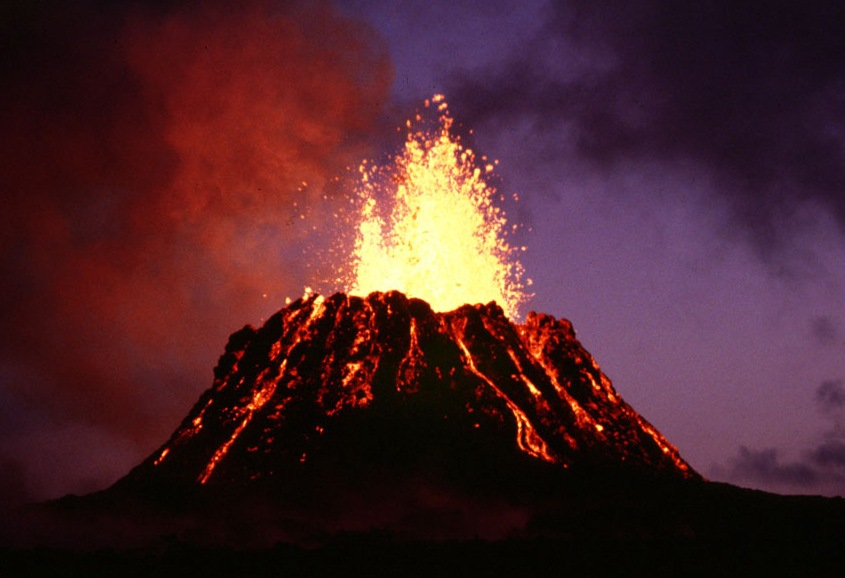
\includegraphics[width=0.55\linewidth]{images/book3/b1-puu-oo-1983.jpg}
\par\smallskip{\small نافورة حمم على مخروط Pu\textquoteleft u~\textquoteleft O\textquoteleft o، على الشقّ الشرقي لكيلاويا، في 29 يونيو 1983، في السنة الأولى من ثوران استمر لعقود: حمم بازلتية حارّة وسائلة تُقذف في نفّاثة وتسقط حول الفوهة. الصورة: G.~E.~Ulrich, U.S. Geological Survey، ملك عام (Wikimedia Commons).}
\label{fig:b1:hotspots:puu-oo}
\end{omfigure}
% ledger: commons:puu-oo, pp1801:kilauea-rate

\begin{history}[إطار ثابت للصفائح]
في 1963 فسّر جون توزو ويلسون جزر هاواي، الأقدم فالأقدم على امتداد خط، بمصدر للحمم محتجز في اللبّ البطيء لخلية حمل في \omterm{def:b1:layered-earth:layers}{الوشاح}، بينما يحمل الجزء العلوي الأسرع من الخلية قاع البحر فوقه. وفي 1971 و\num{1972} جعل دبليو. جيسون مورغان ذلك المصدر عمودًا، قطره نحو \qty{150}{km}، يصعد من أدنى \omterm{def:b1:layered-earth:layers}{الوشاح}، فيكاد يكون ثابتًا بينما تتحرك الصفائح فوقه؛ وسرعان ما بيّنت تجارب الخزانات شكل مثل هذا العمود. وصارت \omterm{def:b1:hotspots:hotspot}{البقع الساخنة} إطارًا تُقاس فيه الصفائح بالنسبة إلى \omterm{def:b1:layered-earth:layers}{الوشاح}، لا بالنسبة إلى بعضها وحده. وبعد نصف قرن صار معروفًا أن الإطار ينجرف، ومنه بقعة هاواي الساخنة وغيرها، لكن ببطء يكفي لأن تُعطي آثار المحيط الهادئ حركة الصفيحة فوق \omterm{def:b1:layered-earth:layers}{الوشاح} لبضع درجات وبضعة سنتيمترات في السنة، كما بيّن تركيب هذا الفصل.
\end{history}
% ledger: hist:plumes, tarduno:emperor

\section{المقاطعات البركانية الكبرى}\label{sec:b1:hotspots:lips}

\begin{definition}[المقاطعة البركانية الكبرى]\label{def:b1:hotspots:lip}
\emph{المقاطعة البركانية الكبرى}\index{المقاطعة البركانية الكبرى} (LIP) تراكم من صخر ناري، معظمه بازلت، لا يتكوّن بالانتشار العادي عند حيد، يغطي أكثر من \qty{e5}{km^2}، ويحوي أكثر من \qty{e5}{km^3}، ويوضع في غضون 50 مليون سنة على الأكثر، معظمه في نبضات مدة كل منها من مليون إلى خمسة ملايين سنة تحمل أكثر من ثلاثة أرباع حجمه. وعلى اليابسة تكون المقاطعات البركانية الكبرى فيضانات بازلتية في معظمها؛ وفي المحيطات، هضاب محيطية.
\end{definition}

تغطي \omterm{def:b1:hotspots:lip}{المقاطعة البركانية الكبرى} النموذجية نحو مليون كيلومتر مربع، وتحوي نحو مليون كيلومتر مكعب من الحمم، معظمها يُقذف في نحو مليون سنة أو أقل. وتتراكم حممها في تدفّقات شبه مستوية، تقطعها التعرية إلى درجات، وهي \emph{الفخاخ} التي سُمّيت بها. ويسرد الجدول أهمّها في آخر 260 مليون سنة.
% ledger: be08:definition, cr03:summary

\begin{omfigure}
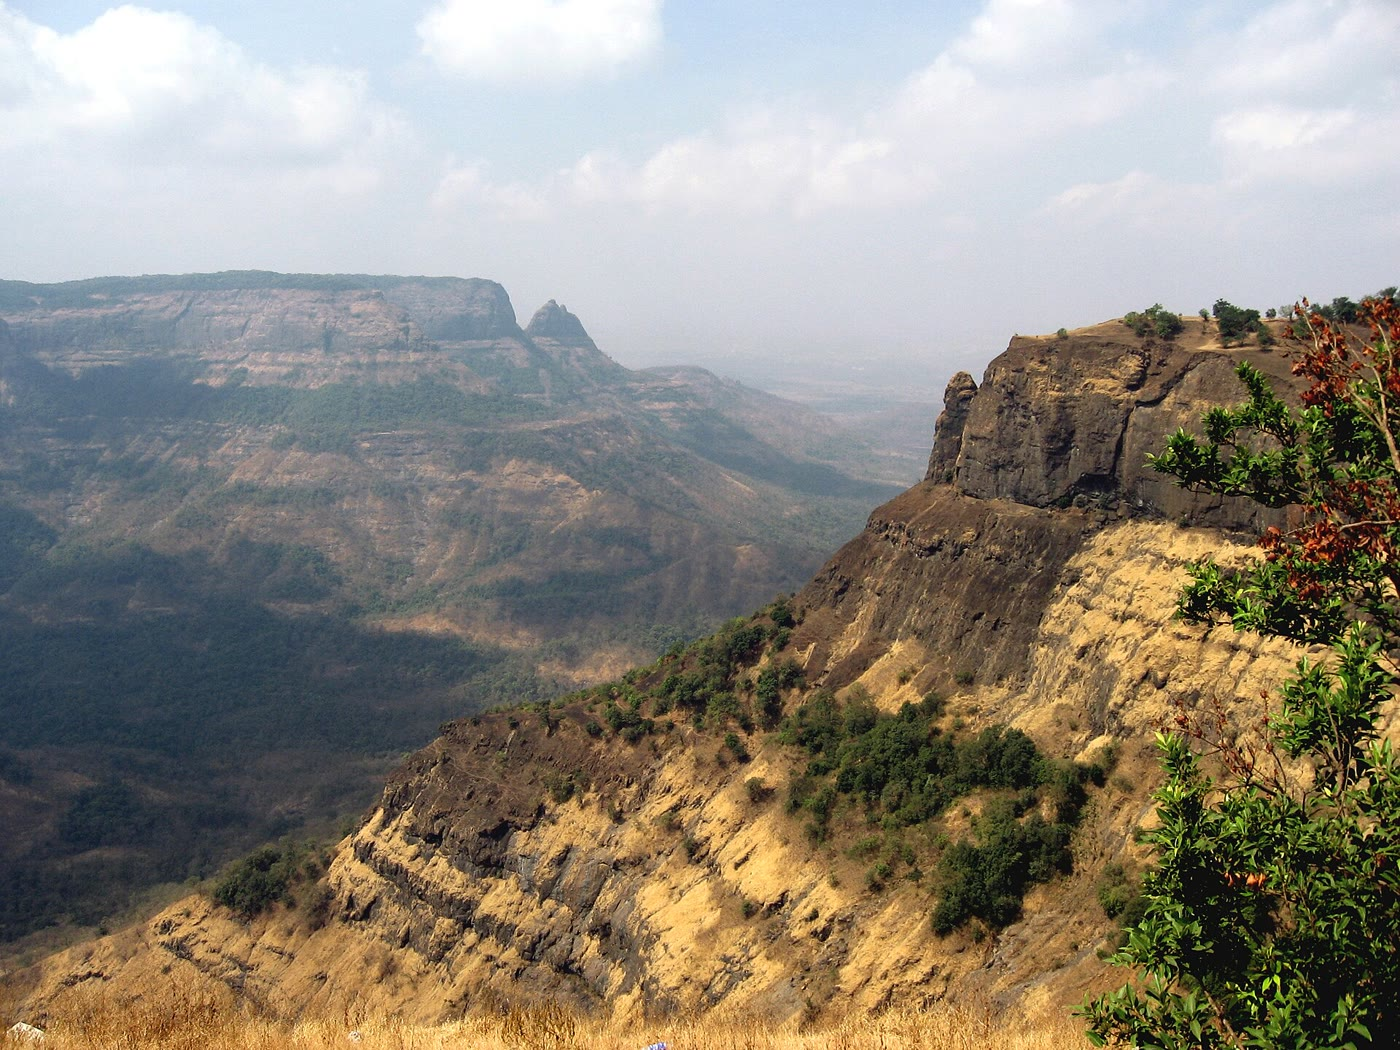
\includegraphics[width=0.55\linewidth]{images/book3/b1-deccan-matheran.jpg}
\par\smallskip{\small جبال غات الغربية قرب ماثيران، في الهند: تلال مسطحة القمم منحوتة في كومة من تدفّقات حمم شبه أفقية لفخاخ الدكن، وطبقاتها المقاومة تصنع درجات المنحدرات. الصورة: Nicholas (Nichalp), CC BY-SA 2.5 (Wikimedia Commons).}
\label{fig:b1:hotspots:deccan}
\end{omfigure}
% ledger: commons:matheran

\begin{center}
\small
\begin{tabular}{llll}
\hline
المقاطعة & العمر (Ma) & المساحة (\unit{Mkm^2}) & الحجم الأول (\unit{Mkm^3})\\
\hline
نهر كولومبيا & \mbox{\textdir TLT 16} & \mbox{\textdir TLT 0.2} & \mbox{\textdir TLT 0.2}\\
إثيوبيا–اليمن & \mbox{\textdir TLT 30} & \mbox{\textdir TLT 0.7} & \mbox{\textdir TLT 1.2}\\
شمال الأطلسي & \mbox{\textdir TLT 61} و\mbox{\textdir TLT 56} & \mbox{\textdir TLT 1.2} & أكثر من \mbox{\textdir TLT 2}\\
الدكن & \mbox{\textdir TLT 65.5} & \mbox{\textdir TLT 0.5} (في وقت ما \mbox{\textdir TLT 1.8}) & \mbox{\textdir TLT 2} إلى \mbox{\textdir TLT 4}\\
أونتونغ جافا & \mbox{\textdir TLT 122} و\mbox{\textdir TLT 90} & \mbox{\textdir TLT 2} & \mbox{\textdir TLT 44} (\omterm{def:b1:layered-earth:layers}{القشرة} كلها)\\
بارانا–إتيندكا & \mbox{\textdir TLT 133} & \mbox{\textdir TLT 1.5} (في وقت ما أكثر من \mbox{\textdir TLT 2}) & أكثر من \mbox{\textdir TLT 2.3}\\
كارو–فيرار & \mbox{\textdir TLT 183} & \mbox{\textdir TLT 3.1} & أكثر من \mbox{\textdir TLT 2.5}\\
الأطلسي الأوسط (CAMP) & \mbox{\textdir TLT 201} & في وقت ما حتى \mbox{\textdir TLT 7} & أكثر من \mbox{\textdir TLT 2}\\
فخاخ سيبيريا & \mbox{\textdir TLT 250} & \mbox{\textdir TLT 0.4} (في وقت ما أكثر من \mbox{\textdir TLT 4}) & أكثر من \mbox{\textdir TLT 3}\\
إيمايشان & \mbox{\textdir TLT 259} & \mbox{\textdir TLT 0.5} (في وقت ما من \mbox{\textdir TLT 2} إلى \mbox{\textdir TLT 5}) & أكثر من \mbox{\textdir TLT 1}\\
\hline
\end{tabular}
\par\smallskip{\small أعمار متوسطة؛ المساحات كما هي اليوم، وكما قُذفت أول مرة حيث يوجد تقدير؛ وأحجام الحمم كما قُذفت أول مرة، باستثناء هضبة أونتونغ جافا، إذ يحسب رقمها قشرتها السميكة كلها. البيانات: V.~Courtillot and P.~Renne (2003).}
\end{center}
% ledger: cr03:table

يفسّر نموذج العمود المرسوم في \cref{sec:b1:hotspots:plumes} الحجم والسرعة معًا: فرأس عمود يبلغ قطره مئات الكيلومترات يصل قاعدة \omterm{def:b1:layered-earth:lithosphere}{الغلاف الصخري}، فيقلّ ضغطه ويذوب، ويغمر السطح؛ ثم يواصل الذيل بناء أثر \omterm{def:b1:hotspots:hotspot}{بقعة ساخنة} عادي. ويُعتقد أن عدة مقاطعات تقع عند الطرف القديم لأثر حيّ: فخاخ الدكن وبقعة ريونيون الساخنة، وبارانا–إتيندكا وتريستان دا كونيا، متصلة بحيد والفيس، وبازلت نهر كولومبيا ويلوستون.
% ledger: cr03:deccan (Reunion hot spot, plume-head model), be08:ojmh (Parana-Etendeka-Walvis-Tristan), pm90:track (Columbia River basalts)

فخاخ الدكن في وسط غرب الهند كومة من تدفّقات الحمم سمكها نحو \qty{2500}{m}، منها ما لا يقل عن \qty{1800}{m} قُذف قرب 65.5 مليون سنة مضت، في زمن أقل بكثير من مليون سنة؛ واليوم تغطي نحو \qty{0.5}{\mega km^2}، وربما \qty{1.8}{\mega km^2} قبل التعرية. وهضبة أونتونغ جافا، في جنوب غرب المحيط الهادئ، أكبر الهضاب المحيطية جميعًا: تغطي نحو \qty{2}{\mega km^2}، وقشرتها، التي يبلغ سمكها نحو \qty{36}{km}، تحوي نحو \qty{44}{\mega km^3} من الصخر الناري. وقد تكون هضبتا مانيهيكي وهيكورانغي، البعيدتان عنها الآن عبر قاع محيط أحدث، تشكّلتا معها كهضبة واحدة. أما المقاطعة المغناطيسية الأطلسية الوسطى، التي قُذفت قبل نحو 201 مليون سنة حين بدأ الأطلسي ينفتح، فهي متناثرة اليوم، كحمم وسدود وعتبات صخرية، عبر أربع قارات: شرق أمريكا الشمالية، وشمال شرق أمريكا الجنوبية، وغرب أفريقيا، وجنوب غرب أوروبا؛ وربما غطّت يومًا حتى \qty{7}{\mega km^2}.
% ledger: cr03:deccan, cr03:table, cr03:ontong-java, be08:ojmh, cr03:camp


تتزامن عدة مقاطعات في الزمن مع الانقراضات الجماعية الكبرى التي تصفها علم الأحياء: فخاخ سيبيريا مع أكبرها جميعًا، عند نهاية البرمي؛ والمقاطعة الأطلسية الوسطى مع نهاية الترياسي؛ وكارو–فيرار مع انقراض في الجوراسي المبكر؛ وإيمايشان مع انقراض في منتصف البرمي؛ وفخاخ الدكن مع نهاية الكريتاسي. وتقع أكبر أربعة انقراضات في آخر 260 مليون سنة كل منها، بأدقّ ما تسمح به التواريخ، على إحدى هذه المقاطعات، ويُعتقد أن صلة سببية هي الأرجح. والآليات المقترحة جوّية: إيروسولات الكبريتات التي تبرّد المناخ لفترة قصيرة، وثاني أكسيد الكربون الذي يسخّنه لمدة أطول بكثير، ومحيطات حُرمت الأكسجين. أما نهاية الكريتاسي، فقد بدأت ثورانات الدكن قبل الاصطدام في تشيكسولوب واستمرت بعده؛ وخلص استعراض لسجلات الحدّ عام 2010 إلى أن الاصطدام أطلق الانقراض.
% ledger: cr03:table, cr03:summary, cr03:deccan, schulte:kpg

لا تحتاج كل البراكين البعيدة عن حدود الصفائح إلى عمود. فتنمو حقول بركانية صغيرة حيث تتمدّد الصفيحة أو تتشقّق، وقد تتغذّى السلاسل التي لا يتقدّم عمرها بوضوح من \omterm{def:b1:layered-earth:layers}{الوشاح} العلوي؛ وهذا هو تطبيق فرضية الصفائح. أما ما تصير إليه الجزر المحيطية بعد أن تتركها \omterm{def:b1:hotspots:hotspot}{البقعة الساخنة}، وهي تغوص وتتآكل وتُكوّن الشعاب، فيعود إلى الكتاب 4.
% ledger: fn03:plate-hypothesis

\section{التمارين}

\begin{exercise}[$\star$]\label{exo:b1:hotspots:1}
(أ) تعلو ماونا كيا \qty{4205}{m} فوق مستوى البحر، وقاع البحر البعيد عن سلسلة هاواي عميق \qty{5274}{m}. كم يعلو البركان فوق ذلك القاع؟ ولماذا يكون ارتفاعه الحقيقي من قاعدته أكبر من ذلك؟ (ب) تحوي ماونا لوا نحو \qty{74000}{km^3}. كم يلزم لبنائه بالإمداد الحالي لكيلاويا، \qty{0.1}{km^3} في السنة، وبالمعدّل المتوسط للسلسلة كلها، \qty{0.025}{km^3} في السنة؟ (ج) أفرغ ثوران بوو-أوو، من 1983 إلى 2002، نحو \qty{0.12}{km^3} في السنة. ما الحجم الكلي لذلك، وما كسره من ماونا لوا؟
% ledger: pp1801:volumes, pp1801:kilauea-supply, pp1801:chain-volume, pp1801:kilauea-rate; 5274 m from hotspots.py
\end{exercise}

\begin{exercise}[$\star$]\label{exo:b1:hotspots:2}
تدور صفيحة فوق \omterm{def:b1:hotspots:hotspot}{البقع الساخنة} بمعدّل \qty{0.92}{\degree\per\Myr}. خذ $R = \qty{6371}{km}$. (أ) عبّر عن $\omega$ بالراديان في كل مليون سنة. (ب) احسب سرعة \omterm{def:b1:hotspots:hotspot}{البقع الساخنة} على \ang{30} و\ang{60} و\ang{90} و\ang{108.0} من القطب، بوحدة \unit{mm.yr^{-1}}. (ج) لماذا تكون سرعة هاواي، عند \ang{108.0}، أقل منها عند \ang{90}؟
\end{exercise}

\begin{exercise}[$\star$]\label{exo:b1:hotspots:3}
(أ) احسب متوسط سمك فخاخ الدكن كما هي اليوم، \qty{1}{\mega km^3} على \qty{0.5}{\mega km^2}، ومتوسط سمك المقاطعة الأطلسية الوسطى، \qty{2}{\mega km^3} على \qty{7}{\mega km^2}. (ب) قارِنه بسمك مقطع الدكن، \qty{2500}{m}. (ج) لماذا لا يقول متوسط سمك المقاطعة الأطلسية الوسطى إلا قليلًا عن سمك كومات حممها؟
% ledger: cr03:table, cr03:deccan, cr03:camp
\end{exercise}

\begin{exercise}[$\star$]\label{exo:b1:hotspots:4}
صخر عمود أحرّ بمقدار \qty{250}{K} من \omterm{def:b1:layered-earth:layers}{الوشاح} المحيط به، له $\alpha = \qty{3.2e-5}{K^{-1}}$ و$\rho_m = \qty{3300}{kg.m^{-3}}$. (أ) بكم يكون أخفّ، بوحدة \unit{kg.m^{-3}}؟ (ب) ما سماكة صخر كهذا، ممتدّ تحت الصفيحة، يحمل أيزوستاتيًا انتفاخًا ارتفاعه \qty{690}{m} تحت البحر ($\rho_w = \qty{1000}{kg.m^{-3}}$)؟
% ledger: herzberg:tp (200-300 K), parsons:plate-model (alpha)
\end{exercise}

\begin{exercise}[$\star\star$]\label{exo:b1:hotspots:5}
تقع بقعتان على خط الاستواء، A عند \ang{0}~ق وB عند \ang{90}~ق، ويمتد أثراهما نحو الغرب تمامًا (سمت \ang{270}). (أ) احسب متجهتي الأثر $\vec t_A$ و$\vec t_B$. (ب) احسب $\vec t_A\times\vec t_B$. (ج) طبّق قاعدة الإشارة في \cref{prop:b1:hotspots:two-tracks}: أين يقع \omterm{def:b1:plate-kinematics:euler-pole}{قطب أويلر}؟ فسّر النتيجة دون حساب. (د) إذا تحركت A بسرعة \qty{50}{mm.yr^{-1}}، فما $\omega$ بالدرجات في كل مليون سنة؟
\end{exercise}

\begin{exercise}[$\star\star$]\label{exo:b1:hotspots:6}
ثلاث \omterm{def:b1:hotspots:hotspot}{بقع ساخنة} لصفيحة واحدة تقع على المسافات $x = R\sin\Delta = 3000$، و\num{5000} و\qty{6000}{km} من محور الدوران، وتتحرك بسرعات 30 و\num{48} و\qty{57}{mm.yr^{-1}}. (أ) ركّب $v = \omega x$ بالمربعات الصغرى، وأعطِ $\omega$ بالراديان وبالدرجات في كل مليون سنة. (ب) احسب البواقي. (ج) لماذا يجب أن يمرّ الخط بالأصل؟
\end{exercise}

\begin{exercise}[$\star\star$]\label{exo:b1:hotspots:7}
يحيط بأثر \omterm{def:b1:hotspots:hotspot}{بقعة ساخنة} فوق صفيحة تتحرك بسرعة \qty{50}{mm.yr^{-1}} انتفاخٌ مقطعه \qty{3e8}{m^2}. خذ $\rho_m - \rho_w = \qty{2300}{kg.m^{-3}}$، و$c_p = \qty{910}{J.kg^{-1}.K^{-1}}$ و$\alpha = \qty{3.2e-5}{K^{-1}}$. (أ) احسب تدفّق طفوه وتدفّق حرارته. (ب) قارنه بهاواي، \qty{3240}{kg.s^{-1}}. (ج) لبقعتين انتفاخ واحد؛ إحداهما تقع تحت صفيحة تتحرك بضعف السرعة. أيّ العمودين أقوى؟
\end{exercise}

\begin{exercise}[$\star\star$]\label{exo:b1:hotspots:8}
على امتداد أثر يلوستون، بدأت ثورانات الكالديرا في حقل ماكديرميت البركاني قبل 16.1 مليون سنة، وفي حقل بيكابو، على بعد نحو \qty{350}{km} شمال شرق، قبل 10.3 مليون سنة؛ ومنذ ذلك الحين تحركت بمقدار $\qty[uncertainty-mode=separate]{2.9 \pm 0.5}{cm}$ في السنة نحو \omterm{def:b1:spherical-astronomy:horizontal}{السمت} \ang{54}. (أ) بأي سرعة متوسطة هاجر البركانية من ماكديرميت إلى بيكابو؟ (ب) قارن السرعتين بسرعة الصفيحة فوق البقعة، \qty[uncertainty-mode=separate]{26 \pm 5}{mm.yr^{-1}} نحو \ang{235}. (ج) هل اتجاه الأثر الفتيّ هو المتوقّع؟ (د) يقع الجزء الأقدم من الأثر في منطقة تمدّدت وهي تمرّ عليها البراكين. كيف يمكن لذلك أن يفسّر الفرق؟
% ledger: pm90:track, data:b3-hotspots
\end{exercise}

\begin{exercise}[$\star\star$]\label{exo:b1:hotspots:9}
يحمل عمود هاواي نحو \qty{9.2e10}{W} من الحرارة الزائدة. (أ) لو خرجت كلها عبر قاع البحر \qty{1000}{km} في \qty{1000}{km} الأقرب إلى \omterm{def:b1:hotspots:hotspot}{البقعة الساخنة}، فبكم كان سيرتفع التدفّق الحراري هناك؟ (ب) قارنه بالزيادة المرصودة، على الأكثر 5 إلى \qty{10}{mW.m^{-2}}. (ج) كم تستغرق الحرارة لتنتشر عبر صفيحة سمكها \qty{100}{km} ($\kappa = \qty{e-6}{m^2.s^{-1}}$)؟ وكم تستغرق الصفيحة لتعبر \qty{1000}{km} بسرعة \qty{92}{mm.yr^{-1}}؟ استنتج.
% ledger: vh89:swell-heat
\end{exercise}

\begin{exercise}[$\star\star\star$]\label{exo:b1:hotspots:10}
تحوي فخاخ الدكن نحو \qty{e6}{km^3} من الحمم. لنفترض أنها أتت من رأس عمود كروي ذاب منه عُشره. (أ) ما حجم الرأس ونصف قطره؟ (ب) لو امتدّ مسطّحًا تحت \omterm{def:b1:layered-earth:lithosphere}{الغلاف الصخري} في قرص سمكه \qty{100}{km}، فما قطره؟ قارِن مساحته بالمساحة التي ربما غطّتها الفخاخ يومًا، \qty{1.8}{\mega km^2}. (ج) لو قُذفت الحمم في مليون سنة، فقارِن معدّلها بالإمداد الحالي لكيلاويا، \qty{0.1}{km^3} في السنة. (د) لماذا يجب أن يكون رأس العمود كبيرًا، بينما الذيل الذي يتبعه ضيّق؟
% ledger: cr03:table, pp1801:kilauea-supply
\end{exercise}

\begin{exercise}[$\star\star\star$]\label{exo:b1:hotspots:11}
بين 81 و\num{47} مليون سنة مضت تحركت بقعة هاواي الساخنة نحو الجنوب بأكثر من \qty{40}{mm.yr^{-1}}. (أ) بأخذ \qty{40}{mm.yr^{-1}}، كم تحركت؟ (ب) لنفترض أن الصفيحة تحركت في الأثناء بسرعة \qty{80}{mm.yr^{-1}} نحو \ang{340} فوق \omterm{def:b1:layered-earth:layers}{الوشاح} العميق. مع $x$ شرقًا و$y$ شمالًا، احسب سرعة الصفيحة بالنسبة إلى البقعة المنجرفة، وسرعتها وسمتها. (ج) بكم بالمئة، وبكم درجة، يكون أثرٌ بُني حينئذٍ مضلِّلًا لحركة الصفيحة فوق \omterm{def:b1:layered-earth:layers}{الوشاح} العميق؟
% ledger: tarduno:emperor
\end{exercise}

\begin{exercise}[$\star\star\star$]\label{exo:b1:hotspots:12}
(أ) يبرد بازلت فيضي حجمه \qty{e6}{km^3} من نحو \qty{1300}{\celsius} إلى حرارة السطح. مع سعة حرارية قدرها \qty{3}{MJ.m^{-3}.K^{-1}}، كم حرارة يطلقها (أهمل الحرارة الكامنة للتبلّر)؟ (ب) موزّعةً على مليون سنة، ما القدرة؟ قارنها بعمود هاواي، \qty{9.2e10}{W}، وبحرارة الأرض الكلية، \qty{47}{TW}. (ج) يسخّن رأس العمود أيضًا قاعدة \omterm{def:b1:layered-earth:lithosphere}{الغلاف الصخري} دون أن يذيب كله. هل قدرة (ب) حدّ أعلى أم حدّ أدنى للحرارة التي يجلبها الرأس؟
% ledger: delaney86:properties (Book 2 row, 2-3 MJ/m3/K), dd10:total; 1300 degC is an exercise value
\end{exercise}

\section{مسألة: مقياس سرعة صفيحة المحيط الهادئ}

\begin{problem}[{مسألة نهاية الأسبوع: قطب صفيحة المحيط الهادئ من أثرين للبقع الساخنة، ومعدّلها من قياس ثالث، واختبار على بقع أخرى، وطفو عمود هاواي وإمداده}]
\label{pb:b1:hotspots:1}
% values: calc/ch15.py; ledger: data:b3-hotspots, data:etopo1, pp1801:kilauea-supply, pp1801:volumes,
% pp1801:chain-volume, delaney86:properties, parsons:plate-model, dd10:total, data:pb2002 (ridge_budget.py), cd87:rate
يسرد مورغان ومورغان بقعة هاواي الساخنة عند \ang{19.0}~ش و\ang{155.2}~غ، بأثر نحو $\ang{304}\pm\ang{3}$ وسرعة \qty[uncertainty-mode=separate]{92 \pm 3}{mm.yr^{-1}}، وبقعة لويزفيل عند \ang{53.6}~ج و\ang{140.6}~غ، بأثر نحو $\ang{316}\pm\ang{5}$ وسرعة \qty[uncertainty-mode=separate]{67 \pm 5}{mm.yr^{-1}}. استعمل المحاور والمتجهات $\vec e$ و$\vec n$ و$\vec t$ في \cref{sec:b1:hotspots:tracks}، مع $R = \qty{6371}{km}$. أعطِ المركبات بأربع منازل عشرية.

\medskip
\noindent\textbf{الجزء الأول --- القطب من أثرين.}
\begin{enumerate}
  \item احسب $\vec r$ و$\vec e$ و$\vec n$ عند هاواي، ثم متجهة الأثر $\vec t_H$.
  \item افعل الشيء نفسه عند لويزفيل: $\vec r_L$ و$\vec e$ و$\vec n$ و$\vec t_L$.
  \item تحقّق من أن $\vec t_H$ متجهة وحدة عمودية على $\vec r_H$.
  \item احسب $\vec t_H\times\vec t_L$ وطوله. ما الزاوية التي تصنعها متجها الأثر؟
  \item اجعل الجداء الاتجاهي متجهة وحدة، وطبّق قاعدة الإشارة في \cref{prop:b1:hotspots:two-tracks}.
  \item أعطِ \omterm{def:b1:spherical-astronomy:geographic}{العرض الجغرافي} \omterm{def:b1:spherical-astronomy:geographic}{والطول الجغرافي} \omterm{def:b1:plate-kinematics:euler-pole}{لقطب أويلر} لصفيحة المحيط الهادئ بالنسبة إلى \omterm{def:b1:hotspots:hotspot}{البقع الساخنة}.
\end{enumerate}

\medskip
\noindent\textbf{الجزء الثاني --- المعدّل.}
\begin{enumerate}[resume]
  \item احسب البعدين الزاويين $\Delta_H$ و$\Delta_L$ من القطب إلى البقعتين الساخنتين.
  \item احسب $(\vec p\times\vec r_L)\cdot\vec t_L$. فسّر لماذا يساوي $\sin\Delta_L$، وماذا تقول إشارته عن الحركة عند لويزفيل.
  \item من سرعة لويزفيل، احسب $\omega$ بالراديان وبالدرجات في كل مليون سنة.
  \item كم تستغرق صفيحة المحيط الهادئ لتدور دورة كاملة حول هذا القطب؟
  \item يقع قطب المربعات الصغرى لآثار المحيط الهادئ الخمسة عشر عند \ang{63.78}~ج و\ang{112.48}~ق، مع \qty{0.92}{\degree\per\Myr}. احسب الزاوية بين القطبين، وقارن المعدّلين.
\end{enumerate}

\medskip
\noindent\textbf{الجزء الثالث --- اختبار على ثلاث \omterm{def:b1:hotspots:hotspot}{بقع ساخنة} أخرى.} يعطي مورغان ومورغان بقعة سوسايتي الساخنة (\ang{18.2}~ج، \ang{148.4}~غ) \qty[uncertainty-mode=separate]{109 \pm 10}{mm.yr^{-1}}، وبيتكيرن (\ang{25.4}~ج، \ang{129.3}~غ) \qty[uncertainty-mode=separate]{90 \pm 15}{mm.yr^{-1}}، وكوب (\ang{46.0}~ش، \ang{130.1}~غ) \qty[uncertainty-mode=separate]{43 \pm 3}{mm.yr^{-1}}.
\begin{enumerate}[resume]
  \item احسب البعد الزاوي من قطب السؤال 6 إلى كل بقعة من \omterm{def:b1:hotspots:hotspot}{البقع الساخنة} الثلاث.
  \item توقّع السرعات الثلاث بمعدّل السؤال 9.
  \item أيّ التوقعات تتفق مع السرعات المقاسة ضمن شكوكها، وأيّها لا يتفق؟
  \item يعطي أثران باتجاهين مختلفين قطبًا دائمًا. فلماذا يكون أثران متوازيين تقريبًا اختيارًا رديئًا؟
\end{enumerate}

\medskip
\noindent\textbf{الجزء الرابع --- العمود ومقياس السرعة.} للانتفاخ الهاواي مقطع \qty{4.83e8}{m^2}. خذ $\rho_m - \rho_w = \qty{2300}{kg.m^{-3}}$، و$c_p = \qty{910}{J.kg^{-1}.K^{-1}}$ و$\alpha = \qty{3.2e-5}{K^{-1}}$.
\begin{enumerate}[resume]
  \item حوّل \qty{92}{mm.yr^{-1}} إلى \unit{m.s^{-1}}، واحسب تدفّق طفو عمود هاواي.
  \item احسب الحرارة الزائدة التي يحملها، وقارنها بالحرارة \qty{47}{TW} التي تغادر الأرض.
  \item تصنع الحيود نحو \qty{21}{km^3} من \omterm{def:b1:layered-earth:layers}{القشرة} كل سنة على طول نحو \qty{67000}{km}. ما طول الحيد الذي يصنع \omterm{def:b1:layered-earth:layers}{قشرة} بقدر ما يُمدّ به كيلاويا، \qty{0.1}{km^3} في السنة؟
  \item بهذا المعدّل، كم يلزم لينمو ماونا لوا، نحو \qty{74000}{km^3}؟
  \item بنت \omterm{def:b1:hotspots:hotspot}{البقعة الساخنة} نحو \qty{2e6}{km^3} من السلسلة في 81 مليون سنة. احسب ناتجها المتوسط، وقارنه بإمداد كيلاويا اليوم.
  \item بالقطب والمعدّل في الجزأين الأول والثاني، احسب السرعة التي يتنبأ بها أثر لويزفيل للصفيحة فوق بقعة هاواي الساخنة.
  \item قارنها بالمقاس \qty[uncertainty-mode=separate]{92 \pm 3}{mm.yr^{-1}}: بكم تختلفان، وبكم من الشكوك المعيارية؟
  \item من أعمار براكين هاواي وجد الكتاب 2 \qty{9.1}{cm} في السنة، ووجد مؤلفو الأعمار، بتركيب السلسلة كلها، \qty{8.6}{cm} في السنة. قارن هذين المتوسطين على عشرات الملايين من السنين بسرعتي \omterm{def:b1:hotspots:hotspot}{البقعة الساخنة}.
  \item بمنزلة عشرية واحدة، وبالسنتيمتر في السنة، ما السرعة التي يعطيها أثر لويزفيل للصفيحة الهادئة فوق بقعة هاواي الساخنة؟
\end{enumerate}
\end{problem}
